% set the song number and formatting
\setcounter{songnum}{106}

%add number image
\newcommand\NumberPic{
\put(0,355){
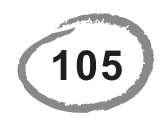
\includegraphics{_images/test.png}
}}

%\AddToShipoutPicture*{\BackgroundPic}
\AddToShipoutPicture*{\NumberPic}



\beginsong{Alegria}[mlby={António Cláudio},
                  %sr={Revelation 5:13},
                  %cr={Public domain.},
                  %arr={my},
                  index={Alegria}]


\begin{wrapfigure}{R}{0.3\textwidth}

\includegraphics[width=0.3\textwidth]{_images/106_Alegria.jpg}
\end{wrapfigure}	 

Intro: G, G$^{7}$, C, Cm, G, D, G, D (G)

\beginverse

\[G]A alegria \[G$^{7}$]está no coração de \[C]quem já conhece \[G]Jesus,
A verdadeira \[Em]paz só tem aquele que \[A]já conhece \[D]Jesus.
O sen\[G]timento mais pre\[G$^{7}$]cioso que \[C]vem do nosso \[Cm]Senhor,
É o \[G]amor, que só \[D]tem quem já conhece \[G]a Jesus.\[C-D]   (repete tudo)
\endverse

\beginchorus
Aleluia, Aleluia, Aleluia, Aleluia. (canon com a estrofe) \\
\endchorus

\beginverse
\chordsoff
O sentimento mais precioso que vem do nosso Senhor, \\
É o amor, \\
Que só tem quem já conhece Jesus. (3x)\\
\endverse

%%%%%%%%%%%%%%%%%%%%%%%%%%%%%%%%%%%%%%%%%%%%%%%%%%%%%%%%%%%%%%%%%%%%%%%%%%%
% print guitar tabs used in this song
%%%%%%%%%%%%%%%%%%%%%%%%%%%%%%%%%%%%%%%%%%%%%%%%%%%%%%%%%%%%%%%%%%%%%%%%%%%
\ifbool{gchords}{					% if the guitar chords are to be printed
\vspace{\gchordsVspace}				% set a vertical space of 10 pt 

\gtabD
\gtabA

}									% end if


%\includegraphics[]{106/106_music.pdf} 
%\begin{figure}[] 
\begin{minipage}[c][\textheight]{\textwidth}
\includegraphics[]{score/106_music.pdf} 
\end{minipage}
%\end{figure}

%%%%%%%%%%%%%%%%%%%%%%%%%%%%%%%%%%%%%%%%%%%%%%%%%%%%%%%%%%%%%%%%%%%%%%%%%%%
% end song latex formating
%%%%%%%%%%%%%%%%%%%%%%%%%%%%%%%%%%%%%%%%%%%%%%%%%%%%%%%%%%%%%%%%%%%%%%%%%%%
\endsong	                   		% end song
